\begin{frame}{Les anniversaires}
  En groupes de 3 ou 4, demandez à votre tour l'anniversaire de chaque personne.
  Par exemple: \\
  \tinygloss{In groups of 3 or 4, take turns asking each person when their birthday is.
  For example:}
  \begin{columns}
    \column{0.5\textwidth}
      \begin{description}
        \item[E1:] Ton anniversaire, c'est quel jour?
        \item[] \tinygloss{Your birthday, it's what day?}
        \item[E2:] C'est le 30 septembre.
        \item[] \tinygloss{It's September 30th.}
      \end{description}
    \column{0.5\textwidth}
      \begin{center}
        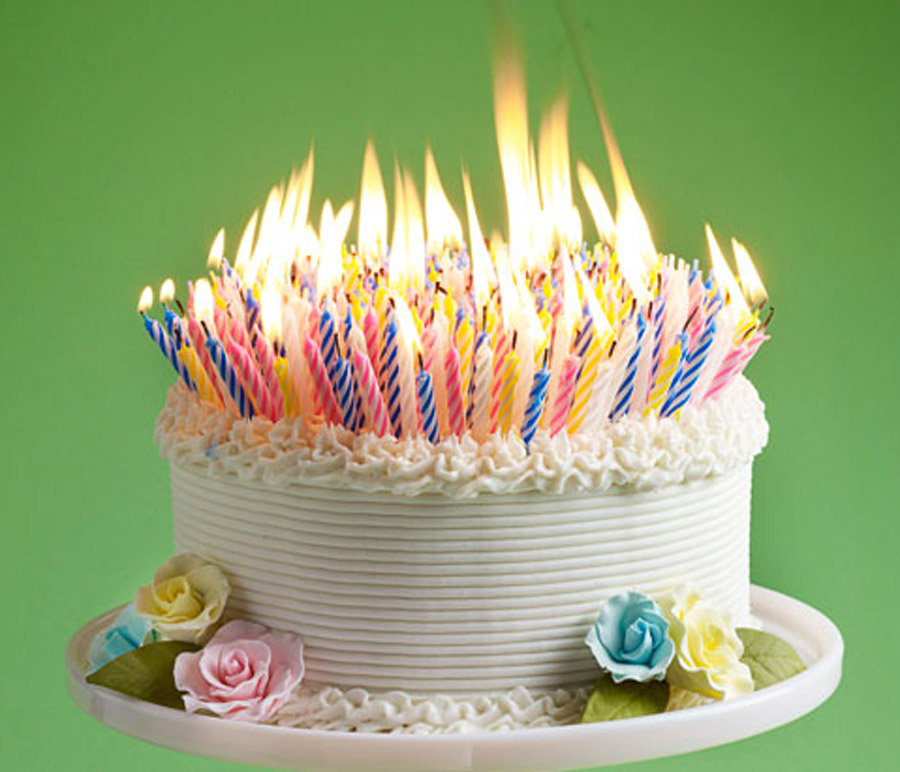
\includegraphics[scale=0.14]{anniversaire.jpg}
      \end{center}
  \end{columns}
\end{frame}
% Follow by asking who has a group member with birthdays on certain days or in
% certain months.